\section{Blades Data}

\subsection{Blades Airfoils}

\begin{figure}[h!]
  \centering
  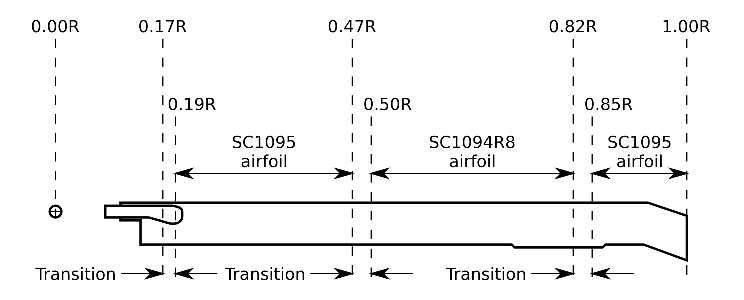
\includegraphics[width=120mm]{eps/uh60_blade.eps}
  \caption{Main rotor blade airfoil section locations \cite{NASA-TM-103985}}
\end{figure}

\subsubsection{SC1094 R8}

\begin{figure}[h!]
  \centering
  \includegraphics[width=127mm]{eps/airfoil_SC1094R8.eps}
  \caption{SC1094 R8}
\end{figure}

\paragraph{Ordinates} ~

\csvreader[
  no head,
  longtable=cccc,
  table head=
    \toprule
    \multicolumn{2}{c}{\bfseries Upper surface} & \multicolumn{2}{c}{\bfseries Lower surface} \\
    x/c & y/c & x/c & y/c \\ \midrule
    \endfirsthead
    \multicolumn{2}{c}{\bfseries Upper surface} & \multicolumn{2}{c}{\bfseries Lower surface} \\
    x/c & y/c & x/c & y/c \\ \midrule
    \endhead,
  before first line={},
  late after line=\\,
  late after last line=\\ \bottomrule \caption{SC1094 R8 \cite{NASA-TP-2003-212265}},
  before reading={},
  after reading={}
]
{csv/airfoil_SC1094R8.csv}
{1=\colxu,2=\colyu,3=\colxl,4=\colyl}
{\colxu & \colyu & \colxl & \colyl}

\paragraph{Aerodynamic Characteristics} ~

\csvreader[
  no head,
  longtable=cccc,
  table head=
    \toprule
    $\alpha$ & $C_L$ & $C_D$ & $C_m$ \\ 
    {[deg]} & {[-]} & {[-]} & {[-]} \\ \midrule
    \endfirsthead
    $\alpha$ & $C_L$ & $C_D$ & $C_m$ \\ 
    {[deg]} & {[-]} & {[-]} & {[-]} \\ \midrule
    \endhead,
  before first line={},
  late after line=\\,
  late after last line=\\ \bottomrule \caption{SC1094 R8 aerodynamic coefficients (XFOIL)},
  before reading={},
  after reading={}
]
{csv/xfoil_out_sc1094r8.csv}
{1=\colaoa,2=\colcz,3=\colcx,4=\colcm}
{\colaoa & \colcz & \colcx & \colcm}

\begin{figure}[p]
  \centering
  \includegraphics[width=140mm]{eps/uh60_blade_sc1094r8_cx.eps}
  \caption{SC1094 R8 drag coefficient}
\end{figure}

\begin{figure}[p]
  \centering
  \includegraphics[width=140mm]{eps/uh60_blade_sc1094r8_cz.eps}
  \caption{SC1094 R8 lift coefficient}
\end{figure}

\begin{figure}[p]
  \centering
  \includegraphics[width=140mm]{eps/uh60_blade_sc1094r8_cm.eps}
  \caption{SC1094 R8 pitching moment coefficient}
\end{figure}

\clearpage
\subsubsection{SC1095}

\begin{figure}[h!]
  \centering
  \includegraphics[width=127mm]{eps/airfoil_SC1095.eps}
  \caption{SC1095}
\end{figure}

\paragraph{Ordinates} ~

\csvreader[
  no head,
  longtable=cccc,
  table head=
    \toprule
    \multicolumn{2}{c}{\bfseries Upper surface} & \multicolumn{2}{c}{\bfseries Lower surface} \\
    x/c & y/c & x/c & y/c \\ \midrule
    \endfirsthead
    \multicolumn{2}{c}{\bfseries Upper surface} & \multicolumn{2}{c}{\bfseries Lower surface} \\
    x/c & y/c & x/c & y/c \\ \midrule
    \endhead,
  before first line={},
  late after line=\\,
  late after last line=\\ \bottomrule \caption{SC1095 \cite{NASA-TP-2003-212265}},
  before reading={},
  after reading={}
]
{csv/airfoil_SC1095.csv}
{1=\colxu,2=\colyu,3=\colxl,4=\colyl}
{\colxu & \colyu & \colxl & \colyl}

\paragraph{Aerodynamic Characteristics} ~

\csvreader[
  no head,
  longtable=cccc,
  table head=
    \toprule
    $\alpha$ & $C_L$ & $C_D$ & $C_m$ \\ 
    {[deg]} & {[-]} & {[-]} & {[-]} \\ \midrule
    \endfirsthead
    $\alpha$ & $C_L$ & $C_D$ & $C_m$ \\ 
    {[deg]} & {[-]} & {[-]} & {[-]} \\ \midrule
    \endhead,
  before first line={},
  late after line=\\,
  late after last line=\\ \bottomrule \caption{SC1095 aerodynamic coefficients \cite{NASA-TM-86719}},
  before reading={},
  after reading={}
]
{csv/SC1095_TM-86719.csv}
{1=\colaoa,2=\colcz,3=\colcx,4=\colcm}
{\colaoa & \colcz & \colcx & \colcm}

\csvreader[
  no head,
  longtable=cccc,
  table head=
    \toprule
    $\alpha$ & $C_L$ & $C_D$ & $C_m$ \\ 
    {[deg]} & {[-]} & {[-]} & {[-]} \\ \midrule
    \endfirsthead
    $\alpha$ & $C_L$ & $C_D$ & $C_m$ \\ 
    {[deg]} & {[-]} & {[-]} & {[-]} \\ \midrule
    \endhead,
  before first line={},
  late after line=\\,
  late after last line=\\ \bottomrule \caption{SC1095 aerodynamic coefficients (XFOIL)},
  before reading={},
  after reading={}
]
{csv/xfoil_out_sc1095.csv}
{1=\colaoa,2=\colcz,3=\colcx,4=\colcm}
{\colaoa & \colcz & \colcx & \colcm}

\csvreader[
  no head,
  longtable=ccc,
  table head=
    \toprule
    $\alpha$ & $C_L$ & $C_D$ \\ 
    {[deg]} & {[-]} & {[-]} \\ \midrule
    \endfirsthead
    $\alpha$ & $C_L$ & $C_D$ \\ 
    {[deg]} & {[-]} & {[-]} \\ \midrule
    \endhead,
  before first line={},
  late after line=\\,
  late after last line=\\ \bottomrule \caption{SC1095 aerodynamic coefficients \cite{NASA-CR-166309}},
  before reading={},
  after reading={}
]
{csv/SC1095_CR-166309.csv}
{1=\colaoa,2=\colcz,3=\colcx}
{\colaoa & \colcz & \colcx}

\clearpage
\newgeometry{margin=1cm}
\thispagestyle{empty}
\begin{sidewaystable}
  \begin{center}
    \scalebox{0.9}
    {
      \begin{tabular}{ c c c c c c c c c c c c }
        \toprule
        $\alpha$ & \multicolumn{11}{c}{$C_L$} \\
        {[deg]} & Ma=0.0 & Ma=0.1 & Ma=0.2 & Ma=0.3 & Ma=0.4 & Ma=0.5 & Ma=0.6 & Ma=0.7 & Ma=0.8 & Ma=0.9 & Ma=10.0 \\ \midrule
        \csvreader[
          column count=12,
          no head,
          late after line=\\
        ]
        {csv/SC1095_CR-166309_cz.csv}
        {}
        {\csvlinetotablerow}
        \bottomrule
      \end{tabular}
    }
    \caption{SC1095 lift coefficient \cite{NASA-CR-166309}}
  \end{center}
\end{sidewaystable}
\restoregeometry

\clearpage
\newgeometry{margin=1cm}
\thispagestyle{empty}
\begin{sidewaystable}
  \begin{center}
    \scalebox{0.9}
    {
      \begin{tabular}{ c c c c c c c c c c c c }
        \toprule
        $\alpha$ & \multicolumn{11}{c}{$C_D$} \\
        {[deg]} & Ma=0.0 & Ma=0.1 & Ma=0.2 & Ma=0.3 & Ma=0.4 & Ma=0.5 & Ma=0.6 & Ma=0.7 & Ma=0.8 & Ma=0.9 & Ma=10.0 \\ \midrule
        \csvreader[
          column count=12,
          no head,
          late after line=\\
        ]
        {csv/SC1095_CR-166309_cx.csv}
        {}
        {\csvlinetotablerow}
        \bottomrule
      \end{tabular}
    }
    \caption{SC1095 drag coefficient \cite{NASA-CR-166309}}
  \end{center}
\end{sidewaystable}
\restoregeometry

\begin{figure}[p]
  \centering
  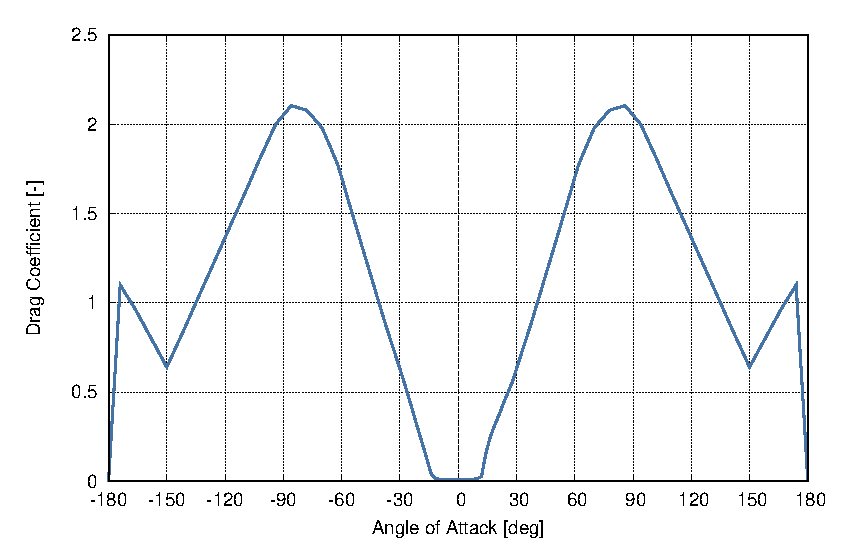
\includegraphics[width=140mm]{eps/uh60_blade_sc1095_cx.eps}
  \caption{SC1095 drag coefficient}
\end{figure}

\begin{figure}[p]
  \centering
  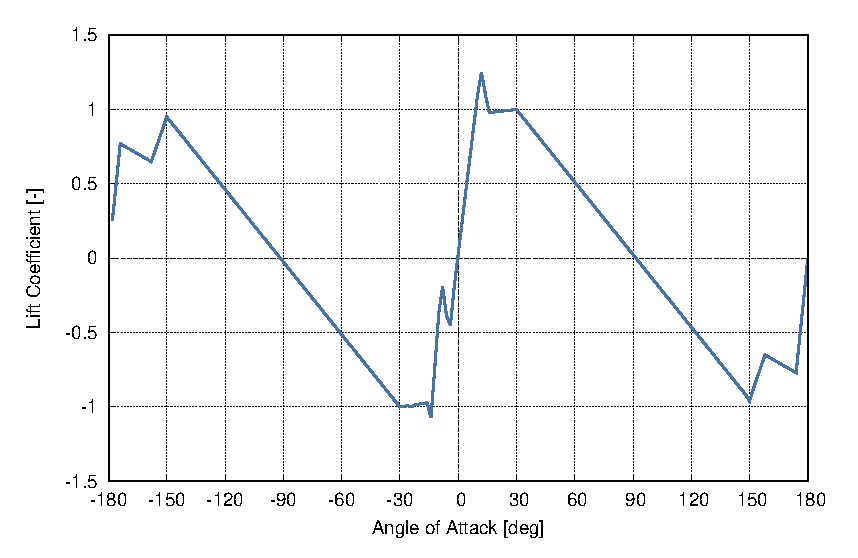
\includegraphics[width=140mm]{eps/uh60_blade_sc1095_cz.eps}
  \caption{SC1095 lift coefficient}
\end{figure}

\begin{figure}[p]
  \centering
  \includegraphics[width=140mm]{eps/uh60_blade_sc1095_cm.eps}
  \caption{SC1095 pitching moment coefficient}
\end{figure}
